%%%%%%%%%%%%%%%%%%%%%%%%%% author.tex %%%%%%%%%%%%%%%%%%%%%%%%%
%
% sample root file for your contribution to an IFIP volume
% published at Springer
%
% Use this file as a template for your own input.
%
%%%%%%%%%%%%%%%%%%%%%%%% Springer-Verlag %%%%%%%%%%%%%%%%%%%%%%%%%%


% RECOMMENDED %%%%%%%%%%%%%%%%%%%%%%%%%%%%%%%%%%%%%%%%%%%%%%%%%%%
\documentclass[ifip]{svmult}

% choose options for [] as required from the list
% in the Reference Guide, Sect. 2.2
\usepackage{epsfig} 
\usepackage{makeidx}         % allows index generation
\usepackage{graphicx}        % standard LaTeX graphics tool
                             % when including figure files
\usepackage{multicol}        % used for the two-column index
\usepackage[bottom]{footmisc}% places footnotes at page bottom
\usepackage{float}
% etc.
% see the list of further useful packages
% in the Reference Guide, Sects. 2.3, 3.1-3.3

\makeindex             % used for the subject index
                       % please use the style sprmidx.sty with
                       % your makeindex program


%%%%%%%%%%%%%%%%%%%%%%%%%%%%%%%%%%%%%%%%%%%%%%%%%%%%%%%%%%%%%%%%%%%%%

\begin{document}

\title*{A Quantitative Analysis of Performance in the Key Parameter in Code Review - Individuation of Defects.}
%code review in software development in cloud-based system }
% Use \titlerunning{Short Title} for an abbreviated version of
% your contribution title if the original one is too long
\author{Dorealda Dalipaj\inst{1}}
% Use \authorrunning{Short Title} for an abbreviated version of
% your contribution title if the original one is too long
\institute{Universidad Rey Juan Carlos, Madrid.
\texttt{dorealda.dalipaj@urjc.es}}
%
% Use the package "url.sty" to avoid
% problems with special characters
% used in your e-mail or web address
%
\maketitle

\textbf{\textit{Abstract -}} Finding and removing defects close to their point of injection remains the main motivation and a key parameter
for review. However, different studies have shown that code review is not performing as expected. They argue that the performance of 
code review is low and that the actual outcome of code reviews in finding errors is less than the expected one. 
Furthermore, another study argues that as many software programs rely on issue reports to correct software errors during maintenance, 
developers spend too much time in identifying the bug
\footnote{In this paper bug and defect refer to the same object.} 
reports
\footnote{In this paper bug report, report and ticket refer to the same object.} 
due to duplicated reports.

The aim of this study is to bring evidence by quantifying the time spent by developers to identify the bugs reports, the time
spent by them to carry out the reviewing process and to bring evidence by quantifying the performance of the very key 
parameter of code review - individuation of bugs.

With the abundance of data and having a diverse set of projects to observe, our case study is focused on 
Open Stack, a cloud computing software. 
Our focus is to have a proof of the rate at which the defects are discovered 
% to what extent developers are actually individuating and fixing bugs 
%while they are applying changes in the code finding 
thus answering if is there any code review providing more value than the others. 

Quantification of the time for identifying bug reports, the review time and the number of bugs fixed during this process, 
% The identification of the bugs report time, review time and the number of bugs fixed during this process, 
are the most fundamental parameters for characterization of performance of the code review and the most important metrics having 
a positive increasing relation with the benefits of this process.


%We focus our case study on a cloud computing software, Open Stack \cite{contribution11}. A developer can contribute to its source code 
%repository using the Launchpad Bugtracking \cite{contribution12} and 
%Gerrit Code Review \cite{contribution13}. First, from Launchpad, we individuate the bug reports that are actually describing a defect, 
%and extracted the needed information to bring statistical evidence on the number of defects that are individuated in Open Stack through the 
%years. Second, we compare the first results to the total number of issues reported, grouped by their different types, 
%to have proof of the rate at which the defects are discovered. And last we bring empirical evidence on the effort spent by developers, 
%by means of time, to carry out the defect individuation process.

%Code review is a well-established and cost-effective way to find defects. 
%Today code review is tool assisted, like from Bug tracking systems that were developed to guide maintenance activities of 
%software developers. Thus today it results time efficient and more lightweight compared to the early software inspections 
%performed in the 80s.  

%However, different studies (\cite{contribution1}, \cite{contribution9}, \cite{contribution20} ) had shown that code review 
%is not performing as expected. 
%They argued that the performance of code review 
%was quite low and that the actual outcome of code review in finding errors was less than expected. Furthermore, another study 
%\cite{contribution10}
%argues that, as many software programs 
%rely on bug reports to correct software errors in maintenance activities, developers spend much time to identify these bug reports. 

%Thus, the aim of this study is to bring evidence by quantifying the performance of the very key parameter of code review: individuation of bugs.
%We focus our case study on a cloud computing software, Open Stack \cite{contribution11}. 
%A developer can contribute to its source code repository using the Launchpad Bugtracking \cite{contribution12} and 
%Gerrit Code Review \cite{contribution13}. First, from Launchpad, we individuate the bug reports that are actually describing a defect, 
%and extracted the needed information to bring statistical evidence on the number of defects that are individuated in Open Stack through the 
%years. Second, we compare the first results to the total number of issues reported, grouped by their different types, 
%to have proof of the rate at which the defects are discovered. And last we bring empirical evidence on the effort spent by developers, 
%by means of time, to carry out the defect individuation process.

\section{Introduction}
\label{sec:1}
% Always give a unique label
% and use \ref{<label>} for cross-references
% and \cite{<label>} for bibliographic references
% use \sectionmark{}
% to alter or adjust the section heading in the running head

Code review, sometimes referred as peer review, employed both in industrial and open source contexts, 
is an activity in which people, other than the author of a code snippet, 
examine it for defects and improvement opportunities.
Code review is characterized \textit{ as a systematic approach to examine a product in detail, 
using a predefined sequence of steps to determine if the product is fit for its intended use}
\cite{contribution14}.

There have been different ways of performing defect detection since its beginning up to nowadays. The formal review or inspection 
according to Fanagan's \cite{contribution15} approach required the conduction of an inspection meeting for actually finding 
defects. Different controlled experiments showed that there were no significant differeneces in the total number of defects found 
when comparing meeting-based with meetingless-based inspections \cite{contribution17, contribution18}. Other 
studies \cite{contribution19} were carried out and proved that more defects were identified with meetingless-based approaches. 
As a result a wide range of mechanisms and techniques of code review were developed. From static analysis 
\cite{contribution3, contribution4, contribution5}, which examines the code in 
the absence of input data and without running the code and is tool based, to modern code review 
\cite{contribution6, contribution7, contribution8}, which aligned with the distributed 
nature of many projects is asynchronous and frequently supporting geographically distributed reviewers. Because of their many uses 
and benefits, code reviews are a standard part of the modern software engineering workflow.

It is generally accepted that quality in software remains a challenge due to defects presence. A major quality issue with 
software is that defects are a byproduct of the complex development process and the ability to develop 
\textit{defect free} software 
remains a big challenge for the software community. 
It is possible to improve the quality of software product by injecting fewer defects or by identifying and 
removing defects injected. 
\\
It is also generally accepted that the performance of software reviews is affected by several factors of the 
defect detection process. So, code review performance is associated with the effort spent to carry out the 
process and the number of defects found. 

Most empirical studies try to assess the impact of specific process settings on performance.
Sources of process variability range from structure (how steps of the inspection 
are organized), inspection inputs (reviewer ability and product quality), 
techniques applied to defect identification that define how each step is carried out), 
context and tool support \cite{contribution16}.  
A controlled experiment by Johnson and Tjahjono \cite{contribution17} showed that \textit{total defects identified, effort spent in the 
process, false positive defects, duplicates} are fundamental variables to analyse when controlling the performance of code review. 

\section{Discussion}
\label{sec:2}

%Static analysis examines code in 
%the absence of input data and without running the code, and can
%detect potential security violations (e.g., SQL injection), runtime errors (e.g., dereferencing a null pointer) and logical
%inconsistencies (e.g., a conditional test that cannot possibly be true). A growing number of projects and companies are concerned about 
%individuating bugs in their code and they are making this process part of their standard build and testing system. 
%According to \cite{contribution2}, Google has incorporated FindBugs into their standard testing and code review process, 
%and has fixed more than 1,000 issues in their internal code base identified by the tool.
%More powerful tools \cite{contribution3}, \cite{contribution4}, \cite{contribution5}, evaluate software in the
%abstract, without executing them or considering a specific input. It has become fairly clear that static analysis
%tools can find important defects in software.

Although code review is used in software engineering primarily for finding defects, several studies argue that 
%they often do not find functionality defects 
the outcome of code reviews in finding errors is less than expected.

Over the past years, a common tool for code review, \texttt{Code Flow}, has achieved wide-spread adoption at Microsoft. 
The functionality of \texttt{CodeFlow} is similar to other review tools such \texttt{Mondrian} \cite{contribution6} 
(adopted at Google), \texttt{Phabricator} 
\cite{contribution7} (adopted at Facebook) or open-source \texttt{Gerrit} \cite{contribution8}.
Two studies have been conducted at Microsoft on code review process, with \texttt{Code Flow} as case study.

The first study \cite{contribution9} took place with professional developers, testers, and managers. 
The results show that, although the top motivation driving code reviews is finding defects, the practice and the 
actual outcomes are less about finding errors than expected: Defect related comments comprise a small proportion, only 14\%, 
and mainly cover small logical low-level issues.
The second study \cite{contribution20} stated that code review do not find bugs. They found that only about 
15\% of the comments provided by reviewers indicate a possible defect, much less functionality issues that should block a 
code submission. 

Another empirical study on the effectiveness of security code review \cite{contribution1}, conducted an experiment on 30 developers. They 
conducted manual code review of a small web application. The web application supplied to the developers had seven known vulnerabilities. 
Their findings concluded that none of the subjects found all confirmed vulnerabilities (they were able to find only 5 out of 7) 
and that reports of false vulnerabilities were significantly correlated with reports of valid vulnerabilities.

A different experiment argued that in large scale software programs where bug tracking systems 
are used developers spend much time to identify the bug reports (mainly due to the excessive number 
of duplicate reports). 

Keeping in mind the above discussion we did these questions:

\begin{itemize}
 \item RQ 1. \textit{What amount of time do developers need to identify bug reports?}
 \item RQ 2. \textit{What is the actual amount of time that developers take in carrying out the review process?}
 \item RQ 3. \textit{Are all the code review tools performing the same in detecting a low number of defects?}
\end{itemize}


With the abundance of data coming from the engineering systems and having a diverse set of projects to observe 
\cite{contribution12, contribution13}, we ask 
if there is any code review providing more value than the others?

To provide answer for the above question we are performing a large empirical study on the actual 213 active projects of Open Stack.
For the purpose of our study, we analyse them divided by the 9 core projects of Open Stack (see \ref{sec:3}), and 
group the rest in the Other Projects category. 

We choose Open Stack because it is a large project that have adopted code reviews on a large 
scale and have a reasonable traceability between commits, review and defects reports.
It uses Launchpad, a bugtracking system for tracking the issue reports, and Gerrit, a lightweight code review tool. Additionally, 
being an open source cloud computing software, it is backed by a global collaboration of developers. It has other flavors worthy of 
additional benefits which influences the outcome, and can bring a different picture from the one in \cite{contribution1}, 
\cite{contribution9}, \cite{contribution20} and \cite{contribution10}. 

In the remainder of this paper, we first describe the necessary background notions for our work (section 3). Next, we describe the 
case study setup (section 4), then present the results of the research questions (section 5). After threats to 
validity and future work (section 6 and section 7), we discuss conclusions (section 8) and we finish with acknowledgements (section 9).

\section{Background}
\label{sec:3}

This section provides background information about the bugtracking and code review environments of Open Stack and the 
tools for obtaining data from their repositories.

Open Stack is a free and open source set of software tools for building and managing cloud computing platforms. 
%It is being employed by 263 users in different industries including: Web/ SaaS/ eCommerce, Information Technology, 
%Healthcare, Cloud Hosting/ MSP/ Telco, Film/ Media/ Gaming, Manifacturing/ Industrial, Retail, Finance ecc.
%The OpenStack Foundation, which oversees both development and community-building around the project, 
%serves more than 30,000 Individual Members from over 170 countries around the world. It is supported by 
%26 platinum and gold members (including AT\&T, Ubuntu, HPE, IBM, Intel, Red Hat, Rackspace, SUSE, Cisco, Dell, Ericson and many 
%5others), 3 infrastructure donors (Rackspace, HPE, OVH Group), and 550 corporate donors and supporting organizations.
%Backed by some of the biggest companies in software development and hosting, as well as thousands of individual community members, 
%OpenStack is the future of cloud computing. 
OpenStack is made up of many different moving parts. Because of its open nature, anyone can add additional components to Open Stack 
to help it to meet their needs. This is why, actually, in Open Stack there are 213 active projects. 
But the OpenStack community has collaboratively identified 9 key components that are a part of 
the \textit{core} of OpenStack, which are distributed as a part of any OpenStack system and officially maintained by the OpenStack 
community: Nova, Swift, Cinder, Neutron, Horizon, Keystone, Glance, Ceilometer, and Heat.
Therefore we will expose the results grouped by the 9 core components of Open Stack and categorise the rest as Other Projects.

Open Stack uses Launchpad, an issue tracking system, which is a repository that enable
users and developers to report defects and feature requests. It allows such a reported issue to be triaged and (if  deemed
important) assigned to team members, to discuss the issue
with any interested team member and to track the history of
all work on the issue. During these issue discussions, team
members can ask questions, share their opinions and help
other team members. Open Stack uses a dedicated reviewing enivornment, 
Gerrit, to  review  patches  and  bug  fixes. It supports with 
lightweight processes for reviewing code changes, i.e., 
to decide whether a developer’s change is safe to
integrate into the official Version Control System (VCS). During this process, 
assigned  reviewers  make  comments
on a code change or ask questions that can lead to a discussion
of  the  change  and/or  different  revisions  of  the  code  change,
before  a  final  decision  is  made  about  the  code  change.  If
accepted, the most recent revision of the code change can enter
the VCS, otherwise the change is abandoned
and the developer will move on to something else.  

%In this paper, we are interested in quantifying:
%\begin{itemize}
% \item the time that developers need to identify a bug report,
% \item the time that developers need to go through the code review process, by measuring the time needed for fixing and merging a change,
% \item and to measure how many bugs (and possibly of what type) where fixed in the
%code changes that successfully  passed in the VCS.
%\end{itemize}

%A developer can contribute to an OpenStack source code repository using Gerrit code review system. Since the Web interface for 
%Gerrit uses Launchpad OpenID single sign-on to identify a developer, an account on bug tracking platform Launchpad is necessary. In 
%addition to the issue and code review repositories, Open Stack adopted modern technology of git for version control system. 
%Furthermore Open Stack is among pioneers for pushing developers to explicitly link code changes to issues and reviews.

To obtain the issue reports and code review data of these ecosystems, we used the data set 
provided by Gonzalez-Barahona et al. \cite{contribution21}.  They  developed the  MetricsGrimoire tool to mine the repositories of
OpenStack, then store the corresponding data into a relational database. We make use of their issue
report and code review data sets \cite{contribution22} to perform our study.


\section{Case Study Setup}
\label{sec:4}

This section explains the methodology used to address our research questions.  
In this paper, we are interested in quantifying:
\begin{itemize}
 \item[$\bullet$] (RQ 1) the time that developers need to identify a bug report in Launchpad,
 \item[$\bullet$] (RQ 2) the time that developers need to go through the code review process in Gerrit,
 %by measuring the time needed for fixing and merging a change,
 \item[$\bullet$] (RQ 3) the bugs (and possibly of what type) that where fixed in the
code changes that were successfully merged to the VCS.
\end{itemize}

Next we discuss the methodology applied for carrying out our study:
\begin{enumerate}
 \item first: the selection of the case study system,
 \item second: how we individuate reports that are actually describing a defect from Launchpad and extracted them for measuring 
 their identification time,
 \item third: how we linked the issues (bug reports from Launchpad) to their review in Gerrit for measuring the time to review,
 \item last: as this is the starting of the PhD, RQ 3 is work in progress, thus we will discuss how we intend to 
 carry it out in Future Work (section \ref{sec:7}).
\end{enumerate}

%   \begin{list}{}{}
%    \item[$\cdot$] prova
%    \item[$\bullet$] prova1
%   \end{list}

\subsection{Selection of Case Study System}
The aim of my PhD, to begin with, is to measure the time that the developers need to identify 
the bug reports in the bugtracking system, 
the time they need to carry out the review, and provide quantitative evidence on the number of bugs detected during the process 
of code review. 
\\
\\
Our case study system choice is Open Stack, because for achieving our aims, we required projects with a
substantial number of commits linked to issue reports and code review. And this is 
readily done in Open Stack.
Furthermore, thanks to MetricsGrimoire tool, we can mine the repositories of Launchpad and Gerrit, which are 
being systematically updated.
What we need to do is to identify the issue reports classified as bugs, link them the respective review and then 
extract the patterns we need for carring out our results.

\subsection{Identifying classified Bug Reports}
\label{sec:4.1}

In Launchpad, besides bugs reports, the developers can work with \textit{specifications} 
(approved design specifications for additions and changes to the project team’s code repositories) 
and \textit{blueprints} (lightweight feature specifications).
Identifying which of the reports have been classified as describing bugs is not a trivial task.
Tickets usually are commented. Reviewers do discuss about having found a bug in a certain report or not. 
But, analysing the comments of a ticket is not the most efficient way for extracting its classification, 
not only because we will not identify 100\% of the tickets but we risk false positives too.
\\
\\
By manual analysis of the tickets and studing the Launchpad work flow, we came accross a pattern 
in the evolution of a report states, with regards to confirming new bugs:

\begin{list}{}{}

\item[$\space$] a) when a ticket, stating a possible bug, is opened in Launchpad, its status is setted to 
\textit{New};
\item[$\space$] b) if the problem described in the ticket is reproduced, the bug is confirmed as genuine and the 
ticket status changes from \textit{New} to \textit{Confirmed};
\item[$\space$] c) only when a bug is confirmed, the status then changes from \textit{Confirmed} to \textit{In Progress} 
the moment when an issue is opened for review in Gerrit.
    
\end{list}
Thus, we analysed the Launchpad repository searching for tickets that match with this pattern. 
These are the tickets that have been classified as bug reports. Once identified, we extracted them in a new repository for further 
inspection.   
\\
\\
Our results showed that, in Launchpad, 57720 tickets out of 88421 have been classified as bugs 
(you can review this results in a python notebook
\footnote{github.com/ddalipaj/CR\_Defect\_Individuation\_Rate/blob/master/finding\_bugs.ipynb} 
that is availabe online). 
Hence 65.3\% of the total tickets in Launchpad are bugs, and an issue for fixing has been opened for them in Gerrit. 
\\
At this point we are able to quantify the time that developers spend on identifying bug reports as the 
distance in time between 
the moment when the ticket is first inserted in Launchpad up to the moment it is 
\textit{Confirmed} as a genuine bug.
\\
You can see the results of the identification of bugs reports in Open Stack divided by the core projects, 
the other projects, and overall Open Stack, in fig. \ref{fig:1} below.

\begin{figure}[H]
\centering
 The percentages of reported issues (tickets) classified as bugs in OpenStack, grouped by projects and last the percentage 
 on the total number of tickets.
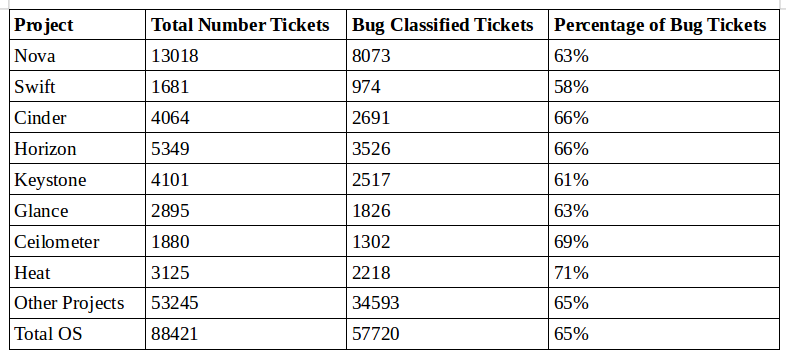
\includegraphics[width=1.0\textwidth,natwidth=786,natheight=360]{bugs_time.png}

\caption{The percentages of reported bugs in OS - From July, 2010 - January, 2016.}
\label{fig:1}       % Give a unique label
\end{figure}


\subsection{Linking the Issue Reports to the Reviews}
\label{sec:4.2}

The next step is to link the tickets that we have already extracted with their respective issue in the code review system.
To detect the links between ticket and reviews, we first referred to the name of the branch on which a code change had 
been made, since some of them follow the naming convention "bug/989868" with "989868" a ticket identifier.
\\
After the extraction, we manually analysed a random number of issues and their respective tickets. We discovered 
that some issues were matched to a ticket like a related artifact, while indeed the issue was reviewing the ticket and 
merging the fixing in the some version of a project (in some cases the same and in others different 
from the one under which the defect was originated). 
The merges in the versions of the same (or even different) project for the preservation of compatibility clearly 
are not elements for measuring the time to review.
\\
To quantify the time that developers do need to carry out the review process
we must be sure take into consideration only merges into the master branch of the projects. 
Thus this selection was clearly erroneus.
\\
We tried \textit{the other way around} approach. Instead of linking reviews to tickets, we linked tickets to reviews using the information
that we find in the comments of the tickets. Whenever a review recieves a proposal for a fix, or a merge for a fix, it is reported in the 
comments of the respective ticket. 
Precisely, a merge comment looks like the following:  
\\
\\
Reviewed:  https://review.openstack.org/100018

Committed: https://git.openstack.org/cgit/openstack/nova/commit
\\
/?id=be58dd8432a8d12484f5553d79a02e720e2c0435

Submitter: Jenkins

Branch:    master ...
\\
\\
Where the first line, clearly, provide us with the link to the issue in Gerrit. 
\\
The first problem that arises in analysing the comments is that, for some ticket, they are a summary of some commit history. 
Therefore, in these cases, we find more than a match with the pattern we are looking for within the body of 
the comment, while the commit itself is not a merge in the master branch of the project that orginated the ticket, 
consequently not the correct result. 
\\
However there is a fixed format of the comments that report a merge (which is the one you can see in the example above).
In this format, the information related to the review is stated at the very begining of the 
comment. Manually analysing the tickets in Launchpad, we have seen that they are found in the first 6 rows of the comment.
\\
Thus the first step is trunking of the comments, so that we extract just the first 6 lines from every one of them. 
Now we are sure we will identify the right review. 
\\
You can review the steps of this process in a python notebook
\footnote{https://github.com/ddalipaj/Analysis\_Tickets\_Issues/blob/master/master\_merge.ipynb}
that is available online. 
\\
At this point we are able to quantify the time to review in OpenStack as the distance in time between the first patch is 
uploaded in Gerrit up to when a fix change is merged to the code base.
\\
The table below (fig. \ref{fig:2}) shows, on the left, the number and percentage of tickets from Launchpad linked with the issues 
in Gerrit that are reviewing them, and on the right, the number and percentage of issues from Gerrit linked with the tickets in 
Launchpad that they are reviewing. 
\\
Our approach was able to link 90.2\% of the tickets from Lauchpad to their corresponding issue, 
and 30.2\% of the issues from Gerrit to the corresponding ticket (the reason behind the results in Gerrit 
is that we are not selecting every merge, but only the ones 
into the master branches).

\begin{figure}[H]
\centering

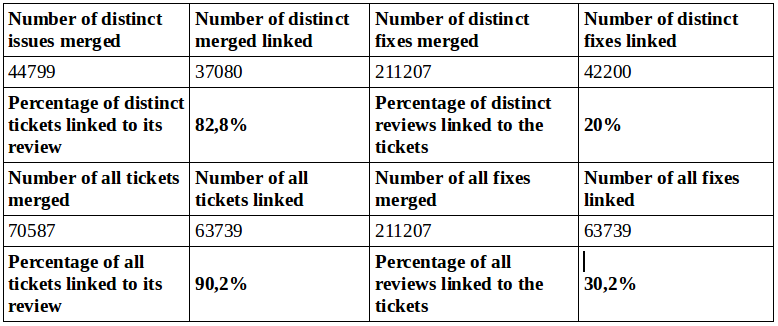
\includegraphics[width=1.0\textwidth,natwidth=778,natheight=326]{t-i.png}

\caption{The percentages of tickets and issues linked with its counterparts in OS - From July, 2010 - January, 2016.}
\label{fig:2}
\end{figure}

\section{Case Study Preliminary Results}
\label{sec:5}

In this section we expose the results that we have obtained for the RQ 1 and 2. As we mentioned before, this is 
the initial phase of the PhD, thus RQ 3 is currently work in progress.
\\
\\
RQ 1. What amount of time do developers need to identify bug reports?
\\
\\
We computed the time for identifying the bug reports as discussed in \ref{sec:4.1}. 
\\
Afterwards, we calculated the median effect size across all Open Stack projects in order to globally rank
the metrics from most extreme effect size, and last the quantiles. 
\\
\\
We discoverd that the median time for identifying a bug report in Open Stack (Launchpad) is 1.96 hours. Additionally, we 
can say that the first quartile is less than 5 minutes, the second quartile is 1.96 hours, the third quartile is 
71.6 hours (less than 3 days), and the interquartile range (IQR) is 71.4 hours (less than 3 days).  
\\
\\
The results are shown in the table below:

\begin{figure}[H]
\centering

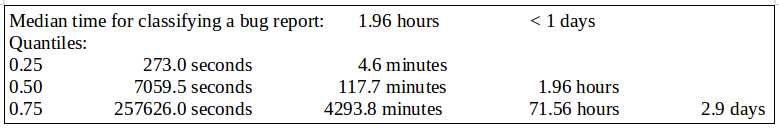
\includegraphics[width=1.0\textwidth,natwidth=779,natheight=129]{t-c.png}

\caption{The median time to classify a bug report accross all projects in Open Stack - From July, 2010 - January, 2016.}
\label{fig:3}       
\end{figure}

RQ 2. What is the actual amount of time that developers take in carrying out the review process?
\\
\\
We computed the time to carry out the review process as discussed in \ref{sec:4.2}.
\\
Again, we calculated the median accross all Open Stack projects. 
\\
\\
We discovered that the median time for reviewing is 52.17 hours (2.2 days). Additionally, we can say that the 
first quartile is 8.21 hours (0.3 days), 
the second quartile is 52.17 hours (2.2 days), the third quartile is 213.75 hours (less than 9 days), 
and the IQR is 205.54 hours (8.6 days).
\\
\\
The results are shown in the table below:

\begin{figure}[H]
\centering

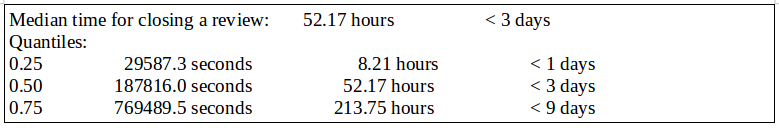
\includegraphics[width=1.0\textwidth,natwidth=779,natheight=129]{t-r1.png}

\caption{The median time to carry out the review process accross all projects in Open Stack - From July, 2010 - January, 2016.}
\label{fig:4} 
\end{figure}

The next table (Fig. \ref{fig:5}) exposes the median of the time to review during various years (from 2011 up to 2015) 
for the 9 core projects of Open Stack, the 
Other Projects category of Open Stack, and over all Open Stack (last row). Additionally the last column exposes the median 
of the time to review over all the history (from July, 2010 to January, 2016) of the above mentioned categories.
\\
\\
We can conclude from the results that in Openstack and the Other Projects category the time to merge is under control.
We can not state the same for some of the core projects. See the trend of the median time in Nova, Cinder, Neutron, Keystone 
and Glance projects.

\begin{figure}[H]
\centering

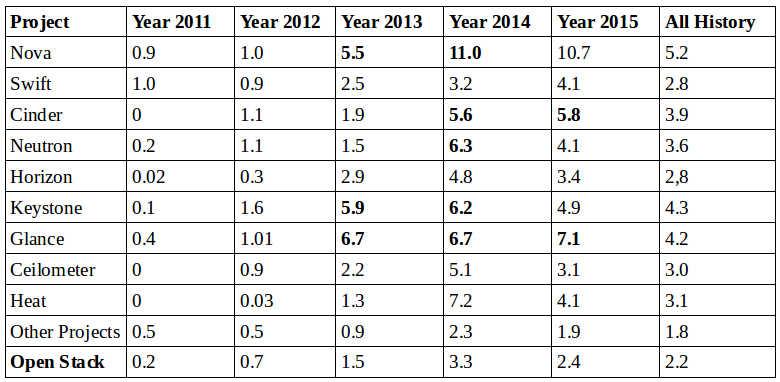
\includegraphics[width=1.0\textwidth,natwidth=781,natheight=381]{gerrit.png}

\caption{The median time to carry out the review process in Open Stack.}
\label{fig:5}       % Give a unique label
\end{figure}

RQ 3. How many bugs (and possibly of what type) where fixed during code review?
\\
\\
The RQ 3 is the topic of the next work in progress.
We are currently working with two elements of the review process that we dispose, the comments and the commit 
analysing both the human discussion and the changes in the code. 

\section{Threats to Validity}
\label{sec:6}

Threats to internal validity concern confounding factors that might influence the results. There
are likely unknown factors that impact defect-detection that we have not analysed and measured yet.
\\
\\
Due to the elaborate filtering that we performed in order to link two repositories (bug repository, 
and code review), the  heuristics  used  to  find  the
relations  between  them  are  not  100\%  accurate,
however  we  used  the  state-of-the-practice  linking  algorithms
at  our  disposal.  Recent  features  in  Gerrit  show  that  clean
traceability  between  version  control  and  review  repositories
is now within reach of each project, hence the available data
for future of this study will only grow in volume.

\section{Future Work}
\label{sec:7} 

Our immediatly future work is to quantify the rate at which bugs are discovered during the code review process.
We are analysing comments and commits not only to identify the changes in the code that are actually fixing bugs, 
but also to find patterns that we can use to automate the process of individuating as precise as possible 
the number of bugs solved during a review. Finally, we can build a tool for monitoring the 
lower and upper bounds of bugs fixed during code review along with other metrics of performance.
\\
There are several other metrics that characterize the 
performance of code review that we would like to investigate. One of them is what influences the time to review 
(fig. \ref{fig:5}).

\section{Conclusion}
\label{sec:8} 

In this paper we emprirically studied the impact of the time for identifying the bug reports and the time to carry out
the review process. We are conducting a study on quantifying the number of bugs fixed during a code review. 
From the preliminary results that we bring into evidence and the future results that we hope to have, we believe that 
our study will open up a variety of research opportunities to continue investigating the impact of collaborative 
characteristics on performance assurance in code review.   

\section{Aknowledgement}

We would like to thank the SENECA EID project, which is funding this research under Marie-Skłodowska Curie Actions.
\\
\\
\\
\\
\\
\\
\textbf{NOTE} 
\\
\\
The preliminary results of this study can be found in three python notebook available online:
\\
\\
1. https://github.com/ddalipaj/CR\_Defects\_Individuation\_Rate/blob/master/
\\
finding\_bugs.ipynb
\\
2. https://github.com/ddalipaj/Analysis\_Tickets\_Issues/blob/master/
\\
master\_merge.ipynb
\\
3. https://github.com/ddalipaj/Reviewing\_Time\_Gerrit/blob/master/
\\
reviewing\_time\_Gerrit.ipynb
\\
\pagebreak














%\subsection{Subsection Heading}
%\label{sec:3}
%Your text goes here.

%\begin{equation}
%\vec{a}\times\vec{b}=\vec{c}
%\end{equation}

%\subsubsection{Subsubsection Heading}
%See Sect.~\ref{sec:1}.

%\paragraph{Paragraph Heading} %
%Your text goes here.

%\subparagraph{Subparagraph Heading.} Your text goes here.%
%
%\index{paragraph}
% Use the \index{} command to code your index words
%
% For tables use
%
%\begin{table}
%\centering
%\caption{Please write your table caption here}
%\label{tab:1}       % Give a unique label
%
% For LaTeX tables use
%
%\begin{tabular}{lll}
%\hline\noalign{\smallskip}
%first & second & third  \\
%\noalign{\smallskip}\hline\noalign{\smallskip}
%number & number & number \\
%number & number & number \\
%\noalign{\smallskip}\hline
%\end{tabular}
%\end{table}
%
%
% For figures use
%
%\begin{figure}
%\centering
% Use the relevant command for your figure-insertion program
% to insert the figure file.
% For example, with the option graphicx use
%\includegraphics[height=4cm]{figure.eps}
%
%\caption{Please write your figure caption here}
%\label{fig:1}       % Give a unique label
%\end{figure}
%
% For built-in environments use
%
%\begin{theorem}
%Theorem text\footnote{Footnote} goes here.
%\end{theorem}
%
% or
%
%\begin{lemma}
%Lemma text goes here.
%\end{lemma}
%
%
% BibTeX users please use
% \bibliographystyle{}
% \bibliography{}
%
% Non-BibTeX users please follow the syntax
% the syntax of "referenc.tex" for your own citations
%%%%%%%%%%%%%%%%%%%%%%%% referenc.tex %%%%%%%%%%%%%%%%%%%%%%%%%%%%%%
% sample references
% "computer science"
%
% Use this file as a template for your own input.
%
%%%%%%%%%%%%%%%%%%%%%%%% Springer-Verlag %%%%%%%%%%%%%%%%%%%%%%%%%%

%
% BibTeX users please use
% \bibliographystyle{}
% \bibliography{}
%
% Non-BibTeX users please use
\begin{thebibliography}{99.}
%
% and use \bibitem to create references.
%
% Use the following syntax and markup for your references
%
% Contributed Works
\bibitem{contribution1} Edmundson, A., Holtkamp, B., Rivera, E., Finifter, M., Mettler, A., Wagner, D. (2013). 
An empirical study on the effectiveness of security code review. In Engineering Secure Software and Systems 
(pp. 197-212). Springer Berlin Heidelberg.

\bibitem{contribution9} Bacchelli Alberto, and Christian Bird. 
"Expectations, outcomes, and challenges of modern code review." 
Proceedings of the 2013 International Conference on Software Engineering. IEEE Press, 2013.

\bibitem{contribution20} Czerwonka Jacek, Michaela Greiler and Jack Tilford. "Code Reviews Do Not Find Bugs."

\bibitem{contribution10} Tao Zhang; Byungjeong Lee "A Bug Rule Based Technique with Feedback for Classifying Bug Reports",  
Computer and Information Technology (CIT), 2011 IEEE 11th International Conference on, On page(s): 336 - 343 

\bibitem{contribution11} IaaS cloud computing of Rackspace Cloud and NASA: https://it.wikipedia.org/wiki/OpenStack and 
https://www.openstack.org

\bibitem{contribution12} Bug Tracking for OpenStack. https://it.wikipedia.org/wiki/Launchpad

\bibitem{contribution13} Gerrit Code Review for OpenStack. //review.openstack.org/Documentation/intro-quick.html

\bibitem{contribution14} D. L. Parnas and M. Lawford. Inspection's role in software quality assurance. In 
Software, IEEE,  vol. 20, 2003. 

\bibitem{contribution15} M. E. Fagan. Design and Code inspections to reduce errors in program development. In IBM Systems Journal 15 
pp. 182-211, 1976. 

\bibitem{contribution17} P. M. Johnson, and D. Tjahjono. Does Every Inspection Really Need a Meeting? In Empirical Software Engineering, vol. 3, 
no. 1, pp. 9-35, 1998. 

\bibitem{contribution18} P. McCarthy, A. Porter, H. Siy et al. An experiment to assess cost-benefits of inspection meetings and their 
alternatives: a pilot study. In Proceedings of the 3rd International Symposium on Software Metrics: From Measurement to Empirical 
Results, 1996. 

\bibitem{contribution19} A. Porter, H. Siy, C. A. Toman et al. An experiment to assess the cost-benefits of code inspections in 
large scale software development. In SIGSOFT Softw. Eng. Notes, vol. 20, no. 4, pp. 92-103, 1995. 

\bibitem{contribution16} D. E. Perry, A. Porter, M. W. Wade. Reducing inspection interval in large-scale software development. In Software 
Engineering, I EEE Transactions on, vol. 28, no. 7, pp. 695-705, 2002. 

\bibitem{contribution2} Broy M (2002) Ayewah, N., Hovemeyer, D., Morgenthaler, J. D., Penix, J., Pugh, W. (2008). 
Using static analysis to find bugs. Software, IEEE, 25(5), 22-29.

\bibitem{contribution3} W. R. Bush, J. D. Pincus, D. J. Sielaff. “A static
analyzer for finding dynamic programming errors,” Softw.
Pract. Exper.
, vol. 30, no. 7, pp. 775–802, 2000.

\bibitem{contribution4} Hallem, D. Park, and D. Engler, “Uprooting software
defects at the source,”
Queue, vol. 1, no. 8, pp. 64–71, 2003.

\bibitem{contribution5} B. Chess and J. West,
Secure Programming with Static
Analysis, 1st ed.  Addison-Wesley Professional, Jul. 2007.

\bibitem{contribution6} N. Kennedy.  How google does web-based code reviews with mondrian.
http://www.test.org/doe/, Dec. 2006.

\bibitem{contribution7} A.  Tsotsis.  Meet  phabricator,  the  witty  code  review  tool  built  inside
facebook.  http://techcrunch.com/2011/08/07/oh-what-noble-scribe-hath-
penned-these-words/, Aug. 2006.

\bibitem{contribution8} Gerrit code review - https://www.gerritcodereview.com/ 

\bibitem{contribution21} J.  M.  Gonzalez-Barahona,  G.  Robles,  and  D.  Izquierdo-Cortazar.   The
metricsgrimoire  database  collection.   In
12th  Working  Conference  on
Mining Software Repositories (MSR)
, pages 478–481, May 2015

\bibitem{contribution22} http://activity.openstack.org/dash/browser/data/db/


\end{thebibliography}

%%%%%%%%%%%%%%%%%%%%%%%%%%%%%%%%%%%%%%%%%%%%%%%%%%%%%%%%%%%%%%%%%%%%%%

%%%%%%%%%%%%%%%%%%%%%%%%%%%%%%%%%%%%%%%%%%%%%%%%%%%%%%%%%%%%%%%%%%%%%%

\printindex
\end{document}





